\section{Architettura}

Per l'architettura dell'applicativo da sviluppare si è deciso di utilizzare
\textit{Model-View-ViewModel}, derivato da \textit{Model-View-Controller}.

\subsection{Viste}
% TODO: Viste non nel senso del pattern
Per garantire l'uniformità e la riusabilità di tutti i componenti delle varie
viste si è deciso di utilizzare per tutti la stessa struttura.

\subsubsection{Caratterizzazione di una vista}
Una vista è caratterizzata da:
\begin{itemize}
  \item Tipo di grafico (scatterplot, parallel coordinates, ecc...).
  \item Impostazioni di rendering.
  \item Associazione degli assi alle dimensioni del grafico.
\end{itemize}

\subsubsection{Logica di Rendering}
\begin{itemize}
  \item Renderer: componente che si occupa di adattare (Adapter pattern) il
    meccanismo di rendering delle varie librerie alla nostra architettura
    specifica, in particolare esso opera sui nostri oggetti di dominio come il 
    dataset già preparato per il render (ad esempio mappati come punti 2 
    dimensionali nello scatterplot) e le sue impostazioni specifiche di 
    rendering (ad esempio lunghezza degli assi x ed y nello scatterplot)
    traducendoli in un formato comprensibile dalla libreria di supporto.
  \item Mapper: componente che si occupa di trasformare il dataset generale nel
    dataset preparato per il render.
\end{itemize}

\begin{figure}[h!]
  \centering
  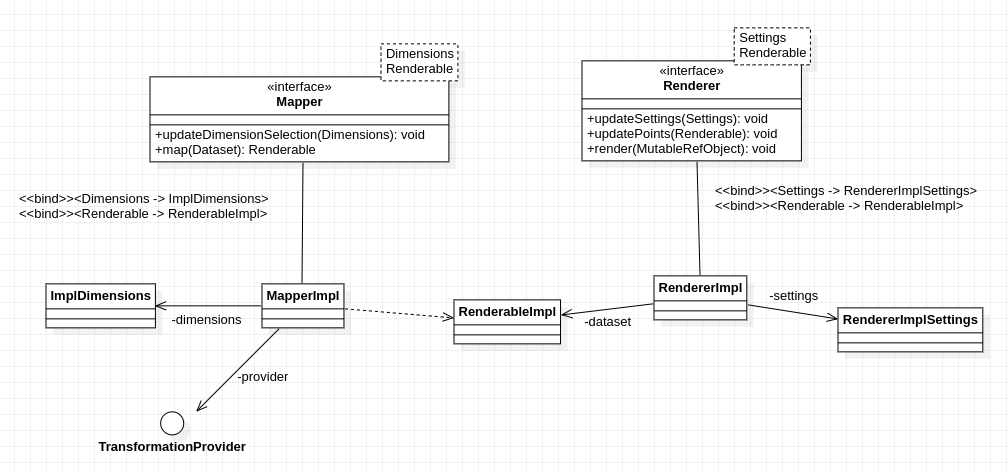
\includegraphics[scale=0.60]{../../assets/classi_uml/modelvista.png}
  \caption{Esempio di implementazione di una vista di tipo \texttt{Impl}.}
\end{figure}
\newpage
\subsubsection{Interazione con l'utente}
L'utente deve poter interagire con l'applicazione per poter modificare
preferenze del grafico specifico, quindi si utilizza mvvm per modellare questa
interazione, il componente verrà generato utilizzando la libreria \texttt{MobX}.

\begin{figure}[h!]
  \centering
  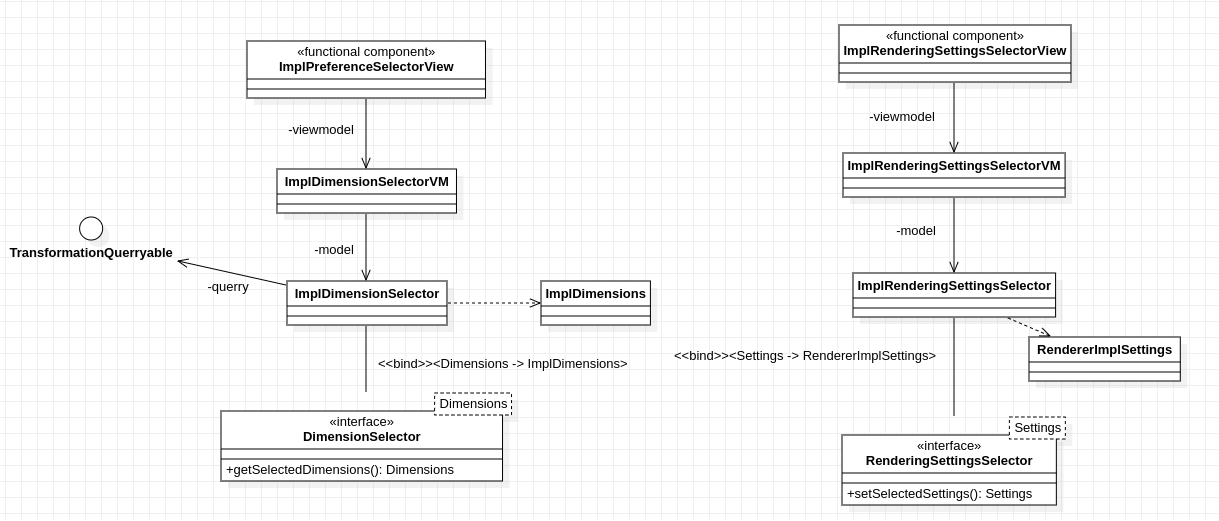
\includegraphics[scale=0.55]{../../assets/classi_uml/modelinterazione.png}
  \caption{Esempio di implementazione dell'interazione di tipo \texttt{Impl}.}
\end{figure}

\subsubsection{Composizione}
Per creare una vista completa sì utilizzerà un componente generico in modo da
favorire la composizione e creazione di nuove tipologie di vista, senza dover
interagire con il codice che si occupa di manipolare il flusso dei dati che data
la nostra architettura risulta essere standard, senza perdere di flessibilità.

\begin{figure}[h!]
  \centering
  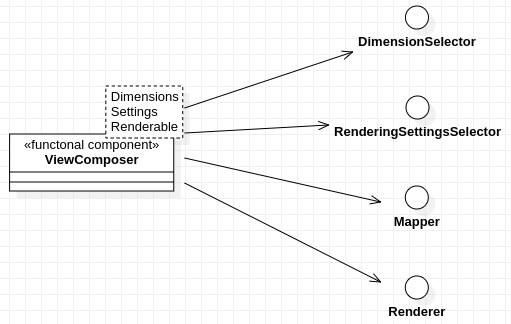
\includegraphics[scale=0.55]{../../assets/classi_uml/comdelcomposer.png}
  \caption{Dimostrazione di composizione generica}
\end{figure}
\newpage

\subsection{Stato dell' applicazione}
L'applicazione ha uno stato con cui tutte le viste interagiscono.
\begin{itemize}
  \item Viste create dall'utente in precedenza.
  \item Trasformazioni sui dati disponibili.
  \item Dataset.
\end{itemize}

\subsubsection{Trasformazioni}
Il transformer è la classe che mantiene traccia di tutte le trasformazioni (cioè
funzioni che trasformano un campo di una entry del dataset in qualcosa che il
renderer è in grado di disegnare). \\
Esso espone 2 interfacce così da segregarne l'uso una è destinata alla ricerca di
trasformazioni (TransformationQuerryable) ed una all' ottenimento tramite
signature (TransformationProvider).
\begin{figure}[h!]
  \centering
  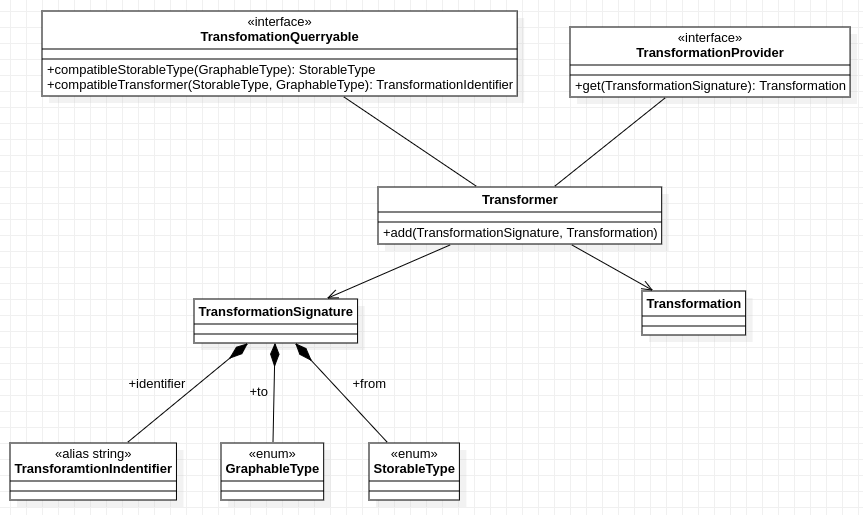
\includegraphics[scale=0.65]{../../assets/classi_uml/modeltransfomer.png}
\end{figure}

% \subsection{Diagrammi dei package}
% \subsection{Diagrammi delle classi}

% \subsubsection{View}

% \begin{figure}[h!]
    % \centering
    % 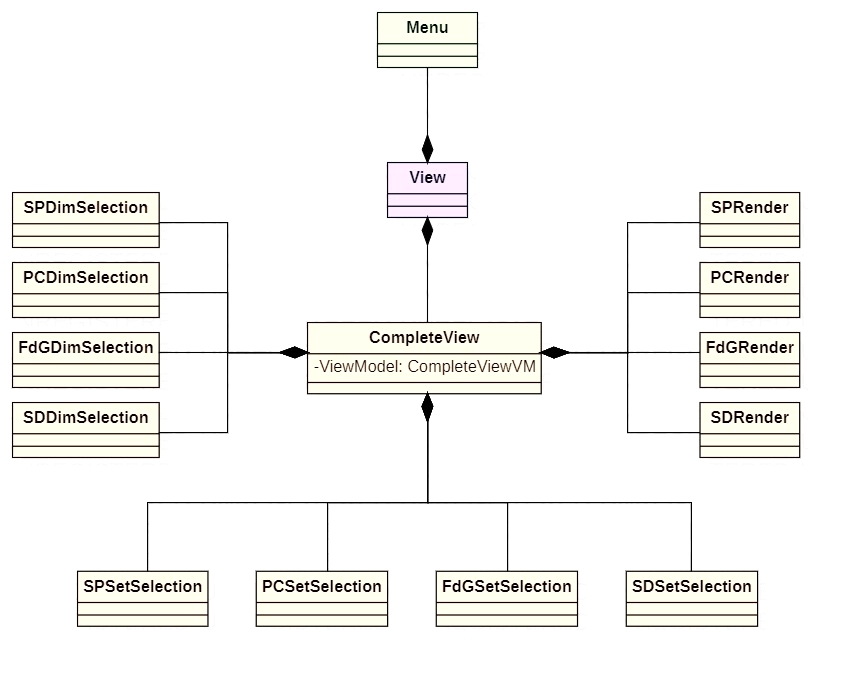
\includegraphics[scale=0.75]{../../assets/classi_uml/View.jpg}
    % \caption{Diagramma delle classi - View}
% \end{figure}
% \newpage
% \subsubsection{Model}

% \begin{figure}[h!]
    % \centering
    % 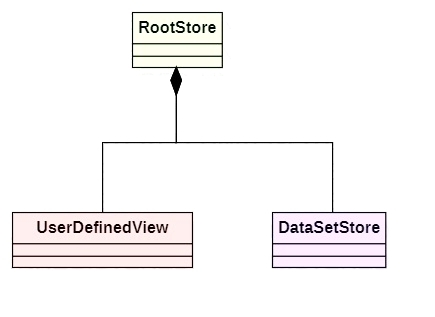
\includegraphics[scale=0.75]{../../assets/classi_uml/Model.jpg}
    % \caption{Diagramma delle classi - Model}
% \end{figure}

% \subsection{Diagrammi di sequenza}
